\documentclass[12pt]{article}
\usepackage[utf8]{inputenc}
\usepackage{parskip}
\usepackage{tabularx}
\usepackage{syntax} % grammar format
% \usepackage{markdown} % inline mark down
\usepackage[color, leftbars]{changebar}

%%%%%%%%%%%%%%%%%%%%%%%%%%%%%%%%%%%%%%%%%%%%%%%%%%%%%%%%%%%%%%%%%%%%%%%%
% Reduce margin
%
% \addtolength{\oddsidemargin}{-.85in}
% \addtolength{\evensidemargin}{-.85in}
% \addtolength{\textwidth}{1in}

% \addtolength{\topmargin}{-.85in}
% \addtolength{\textheight}{1in}

% Page format commands:
% Override normal article margins,
% making the margins smaller
\setlength{\textwidth}{6.5in}
\setlength{\textheight}{9in}
\setlength{\oddsidemargin}{0in}
\setlength{\evensidemargin}{0in}
\setlength{\topmargin}{-0.5in}

\setlength{\parindent}{0pt}

\setlength{\grammarparsep}{20pt plus 1pt minus 1pt} % increase separation between rules
\setlength{\grammarindent}{10em} % increase separation between LHS/RHS 
%%%%%%%%%%%%%%%%%%%%%%%%%%%%%%%%%%%%%%%%%%%%%%%%%%%%%%%%%%%%%%%%%%%%%%%%


%%%%%%%%%%%%%%%%%%%%%%%%%%%%%%%%%%%%%%%%%%%%%%%%%%%%%%%%%%%%%%%%%%%%%%%%
% Math Symbols
\usepackage{mathtools}
\usepackage{amssymb}
% \usepackage{epsfig}
\usepackage{amsmath,amsthm}
\usepackage{amscd,amsxtra,latexsym}


% add floor and ceiling symbol. Usage: \ceil*{}, \floor*{}
% \DeclarePairedDelimiter\ceil{\lceil}{\rceil}
% \DeclarePairedDelimiter\floor{\lfloor}{\rfloor}

% multiset \langle ... \rangle
\def\multiset#1#2{\ensuremath{\left(\kern-.3em\left(\genfrac{}{}{0pt}{}{#1}{#2}\right)\kern-.3em\right)}}



%%%%%%%%%%%%%%%%%%%%%%%%%%%%%%%%%%%%%%%%%%%%%%%%%%%%%%%%%%%%%%%%%%%%%%%%


%%%%%%%%%%%%%%%%%%%%%%%%%%%%%%%%%%%%%%%%%%%%%%%%%%%%%%%%%%%%%%%%%%%%%%%%
% Code Sample Styling

% use \lstinline! (inline text) ! or \begin{lstlisting} text block \end{lstlisting}
\usepackage{listings}

\usepackage{color}
\definecolor{light-gray}{gray}{0.97} % shade of grey
\definecolor{dkgreen}{rgb}{0,0.6,0}
\definecolor{gray}{rgb}{0.5,0.5,0.5}
\definecolor{mauve}{rgb}{0.58,0,0.82}

% \begin{lstlisting}[...] ... \end{lstlisting}
\lstset{frame=none,
    % language=LISP,
    aboveskip=3mm,
    belowskip=3mm,
    stepnumber=0, % set to 0 if you don't like line nums
    showstringspaces=false,
    columns=flexible,
    basicstyle={\small\ttfamily},
    numbers=left,
    numberstyle=\color{black},
    keywordstyle=\color{blue},
    commentstyle=\color{dkgreen},
    stringstyle=\color{mauve},
    backgroundcolor=\color{light-gray},
    breaklines=true,
    breakatwhitespace=false,
    tabsize=2
}



%%%%%%%%%%%%%%%%%%%%%%%%%%%%%%%%%%%%%%%%%%%%%%%%%%%%%%%%%%%%%%%%%%%%%%%%


%%%%%%%%%%%%%%%%%%%%%%%%%%%%%%%%%%%%%%%%%%%%%%%%%%%%%%%%%%%%%%%%%%%%%%%%
\usepackage{xcolor}
%% https://tex.stackexchange.com/questions/401750/quick-and-short-command-for-coloring-one-word
\newcommand\shorthandon{\catcode`@=\active \catcode`^=\active \catcode`*=\active }
\newcommand\shorthandoff{\catcode`@=12 \catcode`^=7 \catcode`*=12 }
\shorthandon
\def@#1@{\textcolor{red}{#1}}%
\def^#1^{\textcolor{blue}{#1}}%
\def*#1{\string#1}
\shorthandoff
%% useage: \textcolor{red}{text here}
% \shorthandon
% This is a @test@ of the ^emergency^ bro*@dcast system.
% \shorthandoff
%%%%%%%%%%%%%%%%%%%%%%%%%%%%%%%%%%%%%%%%%%%%%%%%%%%%%%%%%%%%%%%%%%%%%%%%


%%%%%%%%%%%%%%%%%%%%%%%%%%%%%%%%%%%%%%%%%%%%%%%%%%%%%%%%%%%%%%%%%%%%%%%%
% Misc
\usepackage{graphicx} % graphics
\usepackage{enumitem} % listing style (bullet lists)

% below helps with trying to get figures in a row
% \usepackage{caption}
% \usepackage{subcaption}

% hyperlink styling
% use \href{} and \url{}, and colors table of contents links
% use \href{} and \url{}
% \label{sec:name}
% \hyperref[label]{text}
\usepackage{hyperref}
\hypersetup{
    colorlinks=true,
    linkcolor=blue, % was previously black
    filecolor=magenta,
    urlcolor=blue,
    pdftitle={groot LRM}
}
\urlstyle{same}

% A command for primes (')
\newcommand{\p}%
    {\ensuremath{^{\prime}}}

% a command for double primes ('')
\newcommand{\pp}%
    {\ensuremath{^{\prime \prime}}}

% A command for the Kleene star
\newcommand{\str}%
    {\ensuremath{^{\star}}}

% a command for the double star
\newcommand{\sstr}%
    {\ensuremath{^{\star\star}}}
%%%%%%%%%%%%%%%%%%%%%%%%%%%%%%%%%%%%%%%%%%%%%%%%%%%%%%%%%%%%%%%%%%%%%%%%



\begin{document}
\title{(g)ROOT \\ Language Reference Manual}

\begin{figure}
    \centering
    
\includegraphics{images/babygroot.PNG}
\end{figure}

\author{Samuel Russo \quad Amy Bui \quad Eliza Encherman \\ Zachary Goldstein \quad Nickolas Gravel}
\date{\today}
\maketitle

    \pagebreak
    %%%%%%%%%%%%%%%%%%%%%%%%%%%%%%%%%%%%%%%%%%%%%%%%%%%%%%%%%%%%%%%%%%%%%%%%
    % Table of Contents
    \setcounter{tocdepth}{3}
    \tableofcontents
    \pagebreak 
    %%%%%%%%%%%%%%%%%%%%%%%%%%%%%%%%%%%%%%%%%%%%%%%%%%%%%%%%%%%%%%%%%%%%%%%%

    %%%%%%%%%%%%%%%%%%%%%%%%%%%%%%%%%%%%%%%%%%%%%%%%%%%%%%%%%%%%%%%%%%%%%%%%
    % \section{This is a section heading with number}
    % \label{sec:start} % section label, use to link withing file
    %                   % \hyperref[sec:start]{text}

    % This is a bullet list:
    % \begin{itemize}
    %     \item Link to \href{https://www.overleaf.com/learn/latex/Hyperlinks}{Overleaf href}
    %     \item url example: \url{https://canvas.tufts.edu/}
    %     \item link to aanother labeled section: \hyperref[sec:hello]{Hello World section}
    % \end{itemize}

    % This is a enumlist (default 1):
    % \begin{enumerate}
    %     \item Inline code: \lstinline!(val x 42)! example.
    %     \item \textsc{Hello World}
    %     \item \texttt{Hello World}
    %     \item \textsf{Hello World}
    %     \item This is \textcolor{red}{very Red}
    %     \item This is \textcolor{blue}{Bluey}
    % \end{enumerate}

    % This is enumlist with alph bullets:
    % \begin{enumerate}[label=\alph*.]
    %     \item $x^2 = y$
    %     \item x = y
    % \end{enumerate}

	% \subsection{Grammar}


	% \begin{grammar}
		
	% 	<statement> ::= <ident> `=' <expr> 
	% 	\alt `for' <ident> `=' <expr> `to' <expr> `do' <statement> 
	% 	\alt `{' <stat-list> `}' 
	% 	\alt <empty> 
		
	% 	<stat-list> ::= <statement> `;' <stat-list> | <statement> 
		
	% \end{grammar}


    % %% start on new page
    % \pagebreak
    % %%%%%%%%%%%%%%%%%%%%%%%%%%%%%%%%%%%%%%%%%%%%%%%%%%%%%%%%%%%%%%%%%%%%%%%%


    % %%%%%%%%%%%%%%%%%%%%%%%%%%%%%%%%%%%%%%%%%%%%%%%%%%%%%%%%%%%%%%%%%%%%%%%%
    % \section{Hello World}
%     \label{sec:hello}

%         \subsection{Hello Subsection example}
%             This is how you include pictures:

%             % \begin{figure}[h]
%             %     \centering
%             %     \includegraphics[width=0.7\linewidth]{FILE_PATH}
%             %     % \caption{} %% optional caption
%             %     \label{fig:FILE_NAME}
%             % \end{figure}

%             % \begin{figure}[h]
%             %     \centering
%             %     
\includegraphics[width=0.2\linewidth]{/images/baby_groot.PNG}
%             %     \caption{Our little mascot}
%             %     \label{fig:im_groot}
%             % \end{figure}
            
%             \begin{figure}[h]
%             	\centering
%             	
\includegraphics[width=0.2\linewidth]{images/gt}
%             	\caption{}
%             	\label{fig:babygroot}
%             \end{figure}
            


%             \subsubsection{Basic Table: This doesn't appeear in contents}
%             \begin{center}
%                 \begin{tabular}{|r|c|l|}
%                     \hline
%                     hrow1 & hrow2 & hrow3 \\
%                     \hline
%                     This is & This is & This is\\
%                     right-aligned & centered & left aligned \\
%                     \hline
%                 \end{tabular}
%             \end{center}

%             \begin{center}
%                 \begin{tabular}{l|l|l}
%                     $\leftarrow$ & $\Leftarrow$ & $\langle x + y \rangle$ \\ 
%                     $\rightarrow$ & $\Rightarrow$ & $| x |$ \\ 
%                     $\downarrow$ & $\Downarrow$ & $\| x^2 \|$ \\
%                     $\leftrightarrow$ & $\uparrow$ & \Bigg( \big( cs107 \big)  \Bigg) \\ 
%                     $\epsilon$ & $\rho$ & \Bigg[ \big[ cs107 \big] \Bigg] \\
%                     $\Sigma$ & $\eta$ & \\ 
%                     $\mu$ & \{ \} & \\
%                 \end{tabular}
%             \end{center}

%         \subsection{Another hello subsection example}

%             \subsubsection{Coding environment without line numbers (default)}
% \begin{lstlisting}
% (val add
%     (lambda (x y) 
%         (+ x y)))
% \end{lstlisting}

%             \subsubsection{Coding environment with line numbers (this can be made default)}
% \begin{lstlisting}[stepnumber=1]
% (val add
%     (lambda (x y) 
%         (+ x y)))
% \end{lstlisting}

%             \subsubsection{Code side-by-side}
% \begin{minipage}[h]{0.5\textwidth}
% \begin{lstlisting}
% (val who 
%     (lambda (i am groot) #t)
% )
% \end{lstlisting}
% \end{minipage}
% \begin{minipage}[h]{0.5\textwidth}
% \begin{lstlisting}
% (val were
%     (lambda (senza) (> 3 0))
% )
% \end{lstlisting}
% \end{minipage}
%     \pagebreak
%     %%%%%%%%%%%%%%%%%%%%%%%%%%%%%%%%%%%%%%%%%%%%%%%%%%%%%%%%%%%%%%%%%%%%%%%%


%% LRM OUTLINE STARTS HERE
%%%%%%%%%%%%%%%%%%%%%%%%%%%%%%%%%%%%%%%%%%%%%%%%%%%%%%%%%%%%%%%%%%%%%%%%
\section{Intro}
\label{sec:intro}

At its core, (g)ROOT is a general-purpose functional programming language.
Its syntax stems from functional languages such as Scheme and other
languages rooted in the Lisp family of programming languages. What sets Groot
apart from other programming languages is its native employment of trees.

Trees are a widely-used, abstract data type that represents a hierarchical branching
structure, with a root value and subtrees of children. In many general-purpose
programming languages, trees are not a built-in feature. This forces the
programmer to implement them from the ground up, which can be a tedious process
for many beginner to intermediate programmers. Groot's built-in tree syntax
abstracts this logic away from the programmer, significantly reducing the
complexity inherent to tree development.

In the Groot programming language, trees are a primitive, immutable type
consisting of an element, sibling and child or a \textit{leaf}, a value
representing an empty tree. This allows programmers to easily pass trees between
functions, akin to passing lists in Lisp-style programming languages. Built-in
functions are also supplied to accomplish many common tree operations. These
language features alleviate the burden of implementing, operating, and
maintaining a tree data structure from the programmer, allowing them to focus on
solving more complex problems.


    \subsection{How to read manual}
    The syntax of the language will be given in BNF-like notation. Non-terminal symbol will be in italic font \emph{like-this}, square brackets [ … ] denote optional components, curly braces \{ … \} denote zero or more repetitions of the enclosed component,  and parenthesis ( … ) denote a grouping.

    \pagebreak
    %% End of Introduction %%%%%%%%%%%%%%%%%%%%%%%%%%%%%%%%%%%%%%%%%%%


    %%%%%%%%%%%%%%%%%%%%%%%%%%%%%%%%%%%%%%%%%%%%%%%%%%%%%%%%%%%%%%%%%%%%%%%%
    \section{Lexical Convention}
    \label{sec:lexcon}
        
        \subsection{Blanks} %%%
        The following characters are considered as \textbf{blanks}: space, horizontal tab (`\texttt{\textbackslash t}'), newline character (`\texttt{\textbackslash n}'), and carriage return (`\texttt{\textbackslash r}'). 

        Blanks separate adjacent identifiers, literals, expressions, and keywords. They are otherwise ignored.
        %%%%%%%%%%%%%%%%%%%%%%%%%%%%%%%%%%%%%%%%%%%%%%%%%%%%%%%%%%%%%%%%%%%%%%%%

        \subsection{Comments}
        Comments are introduced with two adjact characters \texttt{(;} and terminated by two adjacent characters \texttt{;)}. Nested comments are currently not allowed. Multiline comments are allowed.\\

% \hspace{1cm}\begin{minipage}[h]{1\textwidth}
\cbcolor{dkgreen}
\cbstart
\begin{lstlisting}
(; This is a comment. ;)

(; This is a 
   multi-lined comment. ;)
\end{lstlisting}
\cbend
% \end{minipage}
        %%%%%%%%%%%%%%%%%%%%%%%%%%%%%%%%%%%%%%%%%%%%%%%%%%%%%%%%%%%%%%%%%%%%%%%%

        \subsection{Identifiers}
        \label{subsec:id}
        Identifiers are sequences of letters, digits, and underscore characters (`\_'), starting with a letter. Letters consist of the 26 lowercase and 26 uppercase characters from the ASCII set.

        \hspace{1cm}\begin{minipage}[h]{1\textwidth}
        \begin{grammar}
            <ident> ::= \texttt{$letter$\ (\ $letter$ | $digit$ | \_ \ )}
            
            <letter> ::= \texttt{a...z\ |\ A...Z }

            <digit> ::= \texttt{0...9 }
        \end{grammar}
        \end{minipage}
        %%%%%%%%%%%%%%%%%%%%%%%%%%%%%%%%%%%%%%%%%%%%%%%%%%%%%%%%%%%%%%%%%%%%%%%%


        \subsection{Integer Literals}
        \label{subsec:intlit}
        An integer literal is a decimal, represented by a sequence of one or more digits, optionally preceded by a minus sign. 

            \hspace{1cm}\begin{minipage}[h]{1\textwidth}
            \begin{grammar}
                <integer-literal> ::= \texttt{[-] $digit$ \{ $digit$ \}}
    
                <digit> ::= \texttt{0...9 }
            \end{grammar}
            \end{minipage}
        %%%%%%%%%%%%%%%%%%%%%%%%%%%%%%%%%%%%%%%%%%%%%%%%%%%%%%%%%%%%%%%%%%%%%%%%

        \subsection{Boolean Literals}
        \label{subsec:boollit}
        Boolean literals are represented by two adjacent characters; the first is the octothorp character (\texttt{\#}), and it is immediately followed by either the \texttt{t} or the \texttt{f} character. 

            \hspace{1cm}\begin{minipage}[h]{1\textwidth}
            \begin{grammar}
                <boolean-literal> ::= \texttt{\# (\ t |\ f\ )}
            \end{grammar}
            \end{minipage}
        %%%%%%%%%%%%%%%%%%%%%%%%%%%%%%%%%%%%%%%%%%%%%%%%%%%%%%%%%%%%%%%%%%%%%%%%

        \subsection{Character Literals}
        \label{subsec:charlit}
        Character literals are a single character enclosed by two \textsf{'} (single-quote) characters.

        %%%%%%%%%%%%%%%%%%%%%%%%%%%%%%%%%%%%%%%%%%%%%%%%%%%%%%%%%%%%%%%%%%%%%%%%

        \subsection{Operators}
        \label{subsec:op}
        All of the following operators are prefix characters or prefixed characters read as single token. Binary operators are expected to be followed by two expressions, unary operators are expected to be followed by one expression. 

        \hspace{1cm}\begin{minipage}[h]{1\textwidth}
            \begin{grammar}

                <operator> ::= (\ \emph{unary-operator} |\ \emph{binary-operator}\ )

                <unary-operator> ::= \texttt{!} |\ \texttt{-}

                <binary-operator> ::= \ \texttt{+\ |\ -\ |\ *\ |\ /\ |\ mod }
                \alt\texttt{==\ |\ \textless\ |\ \textgreater\ |\ $\leq$ |\ $\geq$\ |\ != }
                \alt\texttt{\&\&\ |\ \textcolor{red}{||} }

            \end{grammar}
            \end{minipage}

        \subsection{Keywords}
        \label{subsec:key}
        The below identifiers are reserved keywords and cannot be used otherwise: \\

\cbcolor{dkgreen}
\cbstart
\begin{lstlisting}
if      val         let
leaf    elm         tree
cld     sib         lambda
\end{lstlisting}
\cbend

        The following character sequence are also keywords: \\

\cbcolor{dkgreen}
\cbstart
\begin{lstlisting}
==      +       &&      >       '
!=      -       ||      mod     #t
<=      *       !       (       #f
>=      /       <       )
\end{lstlisting}
\cbend

    \pagebreak
    %% End of Lexical Convention %%%%%%%%%%%%%%%%%%%%%%%%%%%%%%%%%%%%%%%%%%%


%%%%%%%%%%%%%%%%%%%%%%%%%%%%%%%%%%%%%%%%%%%%%%%%%%%%%%%%%%%%%%%%%%%%%%%%
\section{Values}
\label{sec:values}

    \subsection{Base Values}

            \subsubsection{Integer numbers}
            Integer values are integer numbers in range from $-2^{32}$ to $2^{32} - 1$, similar to LLVM's integers, and may support a wider range of integer values on other machines, such as $-2^{64}$ to $2^{64} - 1$ on a 64-bit machine.

            \subsubsection{Boolean values}
            Booleans have two values. \texttt{\#t} evaluates to the boolean value \texttt{true}, and \texttt{\#f} evaluates to the boolean value \texttt{false}.

            \subsubsection{Characters}
            Character values are 8-bit integers between 0 and 255, and follow ASCII standard.

        \subsection{Functions}
        Functional values are mappings from values to value.

        % \subsection{Leaf}

        \subsection{N-Ary Tree Compound Type}
        A core feature of (g)ROOT is its n-ary tree compound value type. Every tree value consists of three components: an element, it's right-immediate sibling, and it's first child. This allows for the convenient implementation of robust recursive algorithms with an arbitrary branching factor.

        Every tree value in (g)ROOT may be either a full tree instance with an element, sibling, and child, or a leaf. The leaf value in (g)ROOT represents the nullary, or empty, tree.

        The tree type in (g)ROOT is modeled after a left-child right-sibling binary tree, where each node contains a reference to its first child and reference to its next sibling. This allows each node in (g)ROOT to have any number of children, while constraining the maximum number of fields per tree instance to three (element, sibling, and child).

        The tree type is very similar in usage to the one-dimensional list type present in many other functional languages, but enforces two additional invariants that empower programmers to shoot themselves in their foot less often.

        \begin{enumerate}
            \item The element of a tree instance may not be itself a tree. An element may be a value of any other type. This enforces a consistent structure among all trees that could be created in (g)ROOT.
            
            \textbf{Note}: it is possible to circumvent this requirement by wrapping a tree instance in a no-args lambda closure. This is a reasonable means of achieving nested data structures as it prevents the accidental creation of nested values; programmers who wrap tree instances in lambda closures likely did not with intention.


            \item Every tree node must have a single immediate sibling and a single immediate child. This forces programmers to think in a purely recursive manner about their solutions.
            
            Trees may be conveniently constructed in-place using the following construction syntax:\\

\cbcolor{dkgreen}
\cbstart
\begin{lstlisting}
'(value left-tree right-tree)
\end{lstlisting}
\cbend

For example:\\

\cbcolor{dkgreen}
\cbstart
\begin{lstlisting}
'(0 leaf (1 (2  (3 leaf leaf) (4 (5 (6 (leaf leaf)) leaf))) (7 (8 leaf leaf) (9 (10 leaf leaf) leaf))))
\end{lstlisting}
\cbend

represents the following tree:
        \begin{figure}[h]
            \centering
            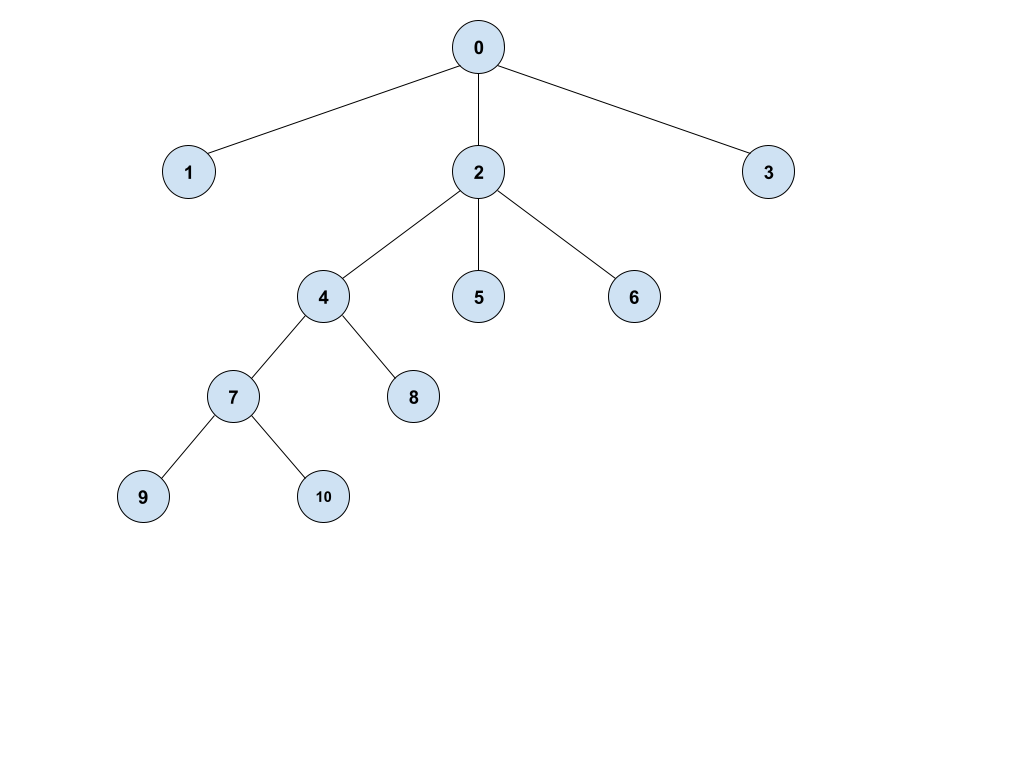
\includegraphics[width=0.9\linewidth]{images/LRMplanning.PNG}
        %     % \caption{} %% optional caption
            \label{fig:tree}
        \end{figure}

        \end{enumerate}

    \pagebreak
    %% End of Values %%%%%%%%%%%%%%%%%%%%%%%%%%%%%%%%%%%%%%%%%%%%%%%%%%%%%%





%%%%%%%%%%%%%%%%%%%%%%%%%%%%%%%%%%%%%%%%%%%%%%%%%%%%%%%%%%%%%%%%%%%%%%%%
\section{Expressions}
\label{sec:expr}

        \hspace{1cm}\begin{minipage}[h]{1\textwidth}
        \begin{grammar}

            <expr> ::= $literal$
            \alt \hyperref[subsec:id]{$ident$}
            \alt \hyperref[subsec:op]{\emph{unary-operator}} $expr$
            \alt (\ \hyperref[subsec:op]{\emph{binary-operator}} $expr$ $expr$)
            \alt (\ \hyperref[subsec:id]{$ident$} \emph{expr-list}  )
            \alt (\ \texttt{val} \hyperref[subsec:id]{$ident$} $expr$  )
            \alt (\ \texttt{let} \hyperref[subsec:id]{$ident$} $expr$ $expr$  )
            \alt (\ \texttt{if} $expr$ $expr$ $expr$  )
            \alt (\ \texttt{lambda} (\ \{$arguments$\} )\ $expr$ )

            <literal> ::=  \hyperref[subsec:intlit]{\emph{integer-literal}} |  \hyperref[subsec:boollit]{\emph{boolean-literal}} | \hyperref[subsec:charlit]{\emph{character}} | \hyperref[subsec:key]{leaf}

            <arguments> ::= $\epsilon$
            \alt \hyperref[subsec:id]{$ident$} :: $arguments$
            

        \end{grammar}
        \end{minipage}

        Expressions are values or parenthetical expressions.

        \subsection{Values}
        see \hyperref[sec:values]{Values}.


        


        \subsection{Parenthetical expressions} Parenthetical expressions (so called because they are always within parentheses) include function application, lambda expressions, global and local definitions, binary and unary operations, and if-statements.

        \subsubsection{Function application}
        Function application in (g)ROOT always returns a value, and is written as the function \texttt{ID} followed by a list of zero or more expressions, which are its arguments. The arguments are not separated from the ID by parentheses. (g)ROOT has first-class functions, therefore functions can be passed as arguments.

        Example:

\cbcolor{dkgreen}
\cbstart
\begin{lstlisting}
(foo)
(foo a b)
\end{lstlisting}
\cbend

        \subsubsection{Lambda Expression}
        Lambda expressions are accomplished with the \texttt{lambda} keyword, a parentheses-enclosed list of 0 or more identifiers as formal arguments, followed by the expression that uses those arguments.

        Example:

\cbcolor{dkgreen}
\cbstart
\begin{lstlisting}
(lambda () #t)
(lambda (x) x), 
(lambda (x y) (+ x y))
\end{lstlisting}
\cbend

        \subsubsection{Global definitions} Global definitions are accomplished using the val keyword, followed by an identifier, followed by the expression which is to be bound to that value.

        Example:

\cbcolor{dkgreen}
\cbstart
\begin{lstlisting}
(val x 4)
(val y (+ x 5))
(val foo (lambda (arg) (* arg arg)))
\end{lstlisting}
\cbend

        Calling a global definition with a preexisting identifier will re-bind that identifier to the new value - currently this is always allowed at the top level, though type-checking may be implemented to ensure it is always of the same type as the previous value.

        \subsubsection{Local definitions} Local definitions are accomplished with the \texttt{let} keyword, followed by the identifier and the expression to be bound to it, followed by the expression that local variable will be used in. 

        Example:

\cbcolor{dkgreen}
\cbstart
\begin{lstlisting}
(let x 4 (+ 2 x))   (; return 6 ;) 
(let x 4 x)         (; return 4 ;) 
\end{lstlisting}
\cbend

        Variables defined within the let binding are not defined outside of it, while variables globally relative to the let can be accessed within it. Since let bindings are a type of expression, this allows for chained let bindings.  

        Example:

\cbcolor{dkgreen}
\cbstart
\begin{lstlisting}
(let x 4 
    (let y 5 
        (let z 9 
            (* x (* y z)))))
\end{lstlisting}
\cbend

        \subsubsection{If-expression}
        If-expressions are currently the only form of control flow in (g)ROOT, and are always formed with the \texttt{if} keyword followed by three expressions (the \emph{condition}, the \emph{true case} and the \emph{false case}). Omission of the false case is a syntax error, and the expressions are not separated by parentheses, brackets, or keywords.
        
        Example:

\cbcolor{dkgreen}
\cbstart
\begin{lstlisting}
(if #t 1 2)
(if (< 3 4) 
    (+ x y) 
    (- x y))
\end{lstlisting}
\cbend

        \subsubsection{Unary operators} Unary operations (used for boolean or signed negation) must not be enclosed in parenthesis - they are accomplished by a unary operator in front of the expression they negate.

        Example:

\cbcolor{dkgreen}
\cbstart
\begin{lstlisting}
-3
-(+ 3 4)
-(if #t 2 3)
-x
\end{lstlisting}
\cbend
        

        Example:

\cbcolor{dkgreen}
\cbstart
\begin{lstlisting}
!#t
!x
!(expr)
\end{lstlisting}
\cbend

        \subsubsection{Binary operators} The general use of binary operators is as follows: (\ \hyperref[subsec:op]{\emph{binary-operator}} $expr_1$ $expr_2$)

        The \textbf{arithmetic operator}s (\ \texttt{+\ ,\ -\ ,\ *\ ,\ /\ ,\ mod }) take two expressions that evaluate to \hyperref[sec:values]{integers}. 

        The \textbf{comparator operators} (\ \texttt{==\ ,\ \textless\ ,\ \textgreater\ ,\ $\leq$ ,\ $\geq$\ ,\ != }) take two expressions that both evaluate to either \hyperref[sec:values]{integers} or \hyperref[sec:values]{booleans}.

        The \textbf{boolean operators} (\ \texttt{\&\& ,\ \textcolor{red}{||} }) take two expressions that evaluate to \hyperref[sec:values]{booleans}.





\pagebreak
%% End of Expressions %%%%%%%%%%%%%%%%%%%%%%%%%%%%%%%%%%%%%%%%%%%


    %%%%%%%%%%%%%%%%%%%%%%%%%%%%%%%%%%%%%%%%%%%%%%%%%%%%%%%%%%%%%%%%%%%%%%%%
    \section{Functions}
    \label{sec:func}

        \subsection{Built-In Functions}
        \textbf{Note}: Throughout this section, the character pair ``tr'' is used as shorthand to represent a tree value, an identifier bound to a tree value.

        There are four built-in functions which are integral to the tree data type:
        \begin{enumerate}
            \item \texttt{elm}

            Usage: \texttt{(elm tr)}

            Purpose: returns the element of the provided tree value \texttt{(tr)}

            \item \texttt{sib}

            Usage: \texttt{(sib tr)}

            Purpose: returns the sinbling tree of the provided tree value \texttt{(tr)}

            \item \texttt{cld}

            Usage: \texttt{(cld tr)}

            Purpose: returns the child tree of the provided tree value \texttt{(tr)}

            \item \texttt{tree}

            Usage: \texttt{(tree ELEMENT SIBLING CHILD)}

            Purpose: constructs a tree value containing the value ELEMENT, with sibling SIBLING and child CHILD.
        \end{enumerate}

        \subsection{Standard Library Functions}
        \textbf{Note}: Throughout this section, the character pair ``tr'' is used as shorthand to represent a tree value, an identifier bound to a tree value.

        The first set of function introduced in the standard library allow for programmers to use some of their beloved list functions present in other languages:
        \begin{enumerate}
            \item \texttt{(cons a b)}
            
            Creates a 1-ary tree approximating the functionality of single-dimensional list in other functional languages.

            \item \texttt{(car tr)}
            
            Extracts the first value in the pair.

            \item \texttt{(cdr tr)}
            
            Extracts the second value in the pair.

            \item \texttt{(null? tr)}
            
            A predicate function that evaluates to true iff the pseudo-list is empty.

            \item \texttt{(val nil leaf)}
            
            A value \texttt{nil} that mirrors the built-in keyword leaf.

            \item \texttt{(append xs ys)}
            
            Append the list of elements in \texttt{ys} to the end of \texttt{xs}.

            \item \texttt{(revapp xs ys)}
            
            Append the list of elements in \texttt{ys} to the reverse of \texttt{xs}.
        \end{enumerate}

        Now some useful tree functions!
        \begin{enumerate}
            \item \texttt{(graft oak fir)}
            
            Appends a sibling tree \texttt{fir} to some other tree \texttt{oak}. The result of calling this function is a new tree in which \texttt{fir} is the rightmost sibling of \texttt{oak}. This function is extremely useful when re-shaping trees.

            \item \texttt{(level-flatten tr)} 
            
            Flattens the provided tree to a 1-ary tree, arranging elements in level-order.

            \item \texttt{(pre-flatten tr)}
            
            Flattens the provided tree to a 1-ary tree, arranging elements in pre-order.
            
            \item \texttt{(post-flatten tr)}
            
            Flattens the provided tree to a 1-ary tree, arranging elements in post-order.
            
            \item \texttt{(map f tr)}
            Maps a function \texttt{f} over every element of the provided tree \texttt{tr}.
            
            \item \texttt{(filter p? tr)}
            
            Constructs a new tree containing only elements that satisfy the predicate function \texttt{p?}, which must return a boolean value.
            
            \item \texttt{(level-fold fn base tr)}
            
            Folds a tree, visiting each element in a level-order traversal. Note that the accumulation function \texttt{fn} must take TWO arguments, the first of which is the current element, and second is the rest of the tree.
            
            \item \texttt{(pre-fold fn base tr)}
            
            Folds a tree, visiting each element in a pre-order traversal. Note that the accumulation function \texttt{fn} must take TWO arguments, the first of which is the current element, and second is the rest of the tree.

            \item \texttt{(post-fold fn base tr)}
            
            Folds a tree, visiting each element in a post-order traversal. Note that the accumulation function \texttt{fn} must take TWO arguments, the first of which is the current element, and second is the rest of the tree.
            
            \item \texttt{(fold fn base tr)}
            
            Folds a tree, in a more intuitively tree-like manner. Note that the accumulation function \texttt{fn} must take THREE arguments: the value of the current node, the sibling accumulator, and the child.accumulator.
            
            \item \texttt{(node-count tr)}
            
            Evaluates to the number of nodes in the provided tree.
            
            \item \texttt{(height tr)}
            
            Evaluates to the height of the provided tree.

        \end{enumerate}

        Higher-Order Functions:
        \begin{enumerate}
            \item \texttt{(curry f)}
            
            Allows for the partial application of a two-argument function.
            
            \item \texttt{(uncurry f)}
            
            Uncurries a previously curried function such that both of its arguments must be provided at the same time.
            
            \item \texttt{(o f g)}
            
            Given two single-argument functions, returns a single function which is the composition of \texttt{f} and \texttt{g}.
            
            \item \texttt{(flip f)}
            
            Given a two argument function, reverses the order in which the arguments are evaluated and passed to the function.
            
            \item \texttt{(flurry f)}
            
            Given a two argument function, reverses the order in which the arguments are evaluated and passed to the function, and allows for the partial application of that function. This function both flips and curries \texttt{f} (hence the fun name).

        \end{enumerate}

    \pagebreak
    %% End of Functions %%%%%%%%%%%%%%%%%%%%%%%%%%%%%%%%%%%%%%%%%%%


    %%%%%%%%%%%%%%%%%%%%%%%%%%%%%%%%%%%%%%%%%%%%%%%%%%%%%%%%%%%%%%%%%%%%%%%%
    \section{Appendix}
    \label{sec:app}

\cbcolor{dkgreen}
\cbstart
\begin{lstlisting}
(; We can define standard list functions with our tree data type! Fun! ;)

(define (cons a b) (tree a leaf (tree b leaf leaf)))
(define (car   tr) (elm tr))
(define (cdr   tr) (cld tr))
(define (nil     ) leaf)
(define (null? tr) (leaf? tree))
   
(; a list function! ;)
(define append (xs ys)
    (if (null? xs)
        ys
        (cons (car xs) (append (cdr xs) ys))
    )
)
   
(; another list function! ;)
(define revapp (xs ys) ; (reverse xs) followed by ys
    (if (null? xs)
        ys
        (revapp (cdr xs) (cons (car xs) ys))
    )
)
   
(; appends a sibling tree (fir) to tree (oak) ;)
(define (graft oak fir)
    (if (leaf? oak)
        fir
        (tree (elm oak) (graft (sib oak) fir) (cld oak))
    )
)
   
(; attempt 4 
   this function flattens a tree, level-order ;)
(define (level-flatten tr)
    (if (leaf? tr)
        leaf
        (tree
            (elm tr)
            leaf
            (level-flatten (graft (sib tr) (cld tr)))
        )
    )
)
\end{lstlisting}
\cbend



flattening functions!

\cbcolor{dkgreen}
\cbstart
\begin{lstlisting}
(; this function flattens a tree, pre-order ;)
(define (pre-flatten tr)
    (if (leaf? tr)
        leaf
        (tree
            (elm tr)
            leaf
            (pre-flatten (graft (cld tr) (sib tr)))
        )
    )
)
   
   
(; this function flattens a tree, post-order ;)
(define (post-flatten tr)
    (if (leaf? tr)
        leaf
        (if (leaf? (cld tr))
            (tree
                (elm tr)
                leaf
                (post-flatten (sib tr)))
            (post-flatten (graft
                                (graft
                                    (cld tr)
                                    (tree (elm tr) leaf leaf))
                                (sib tr))
            )
        )
    )
)
\end{lstlisting}
\cbend


Let's create some higher order functions! Yay!

\cbcolor{dkgreen}
\cbstart
\begin{lstlisting}
(define (curry   f)   (lambda (x)   (lambda (y) (f x y))))
(define (uncurry f)   (lambda (x y) ((f x) y)))
(define (o       f g) (lambda (x)   (f (g x))))
(define (flip    f)   (lambda (x)   (lambda (y) (f y x))))


\end{lstlisting}
\cbend



function: (flurry func)
\begin{itemize}
    \item precondition:
    
    func is a function that takes exactly two args

    \item evalutation: 
    
    evaluates to a curried form of func, where:
        \begin{enumerate}
            \item the first value passed to the curried function is treated as the second argument to (func).
            \item the second value passed to the curried function is treated as the first argument to (func).
        \end{enumerate}

    \item note: flurry is a contraction of ``flip \& curry'', and I'm very proud of the wordplay there.
\end{itemize}


\cbcolor{dkgreen}
\cbstart
\begin{lstlisting}
(define flurry (func)
    (curry (lambda (a b) (func b a)))
)


(; mapping function! ;)
(define (map f tr)
    (if (leaf? tr)
        leaf
        (tree
            (f (elm tr))
            (map f (sib tr))
            (map f (cld tr))
        )
    )
)
   

(; filter function! ;) 
(define filter (p? tr)
    (if (leaf? tr)
        leaf
        (if (p? (elm tr))
            (tree (elm tr) (filter p? (sib tr)) (filter p? (cld tr)))
            (filter p? (graft (cld tr) (sib tr)))
        )
    )
)
   
   
   

(; folding functions! ;) 

(; attempt 4 
   this function folds a tree, level-order ;) 
(define (level-fold fn base tr)
    (if (leaf? tr)
        base
        (fn
            (elm tr)
            (level-fold (graft (sib tr) (cld tr)))
        )
    )
)
   
(; this function folds a tree, pre-order ;) 
(define (pre-fold fn base tr)
    (if (leaf? tr)
        base
        (fn
            (elm tr)
            (pre-fold (graft (cld tr) (sib tr)))
        )
    )
)
   
(; this function folds a tree, post-order ;) 
(define (post-fold fn base tr)
    (if (leaf? tr)
        base
        (if (leaf? (cld tr))
            (fn (elm tr) (post-fold (sib tr)))
            (post-fold (graft
                            (graft (cld tr) (tree (elm tr) leaf leaf))
                                (sib tr)
                        )
            )
        )
    )
)
   
(; once we implement first-class functions, we 
   should find that the behaviors of these three
   functions are exactly equivalent to their
   lower-class cousins ;) 
(define (level-fold-flatten tr) (level-fold cons nil tr))
(define (pre-fold-flatten   tr) (pre-fold   cons nil tr))
(define (post-fold-flatten  tr) (post-fold  cons nil tr))

(; this function folds a tree, in a more intuitively 
   tree-like manner
   fn must take in three params: 
   - the current value   
   - the sibling accumulator
   - the child accumulator ;)     
(define (fold fn base tr)
    (if (leaf? tr)
        base
        (fn
            (elm tr)
            (fold fn base (sib tr))
            (fold fn base (cld tr))
        )
    )
)
   
   

(; some more fun folding functions! ;) 
(define (node-count tr)
    (pre-fold (lambda (elem count) (+ 1 count)) 0 tr)
)
   
(; this uses the tree fold to calculate the height! ;) 
(define (height tr)
    (fold
        (lambda (elem clds sibs) (+ 1 (max clds sibs)))
        0 tr
    )
)

(define (height-no-fold tr)
    (if (leaf? tr)
        0
        (max (height (sib tr)) 
            (+ 1 (height (cld tr)))
        )
    )
)
\end{lstlisting}
\cbend

    % \pagebreak
    %% End of Appendix %%%%%%%%%%%%%%%%%%%%%%%%%%%%%%%%%%%%%%%%%%%



\end{document}